\section{Natural Language Processing}
Human language is a symbolic system aimed at the transmission of meaning.
The symbols of a language can be encoded in various ways: sounds gestures writing. \\
\vspace{1em}
NLP is concerned with creating an algorithm that can understand natural language (knowledge acquisition) and communicate with humans.
This can help in various contexts such as translating text,answering questions and creating summaries.
However, understanding natural language is complicated given its ambiguous nature.

\subsection{NLP Levels}
There are several levels of NLP.
The format must be made understandable to the algorithm.
\begin{center}
    \begin{tabular}{c}
        \\ 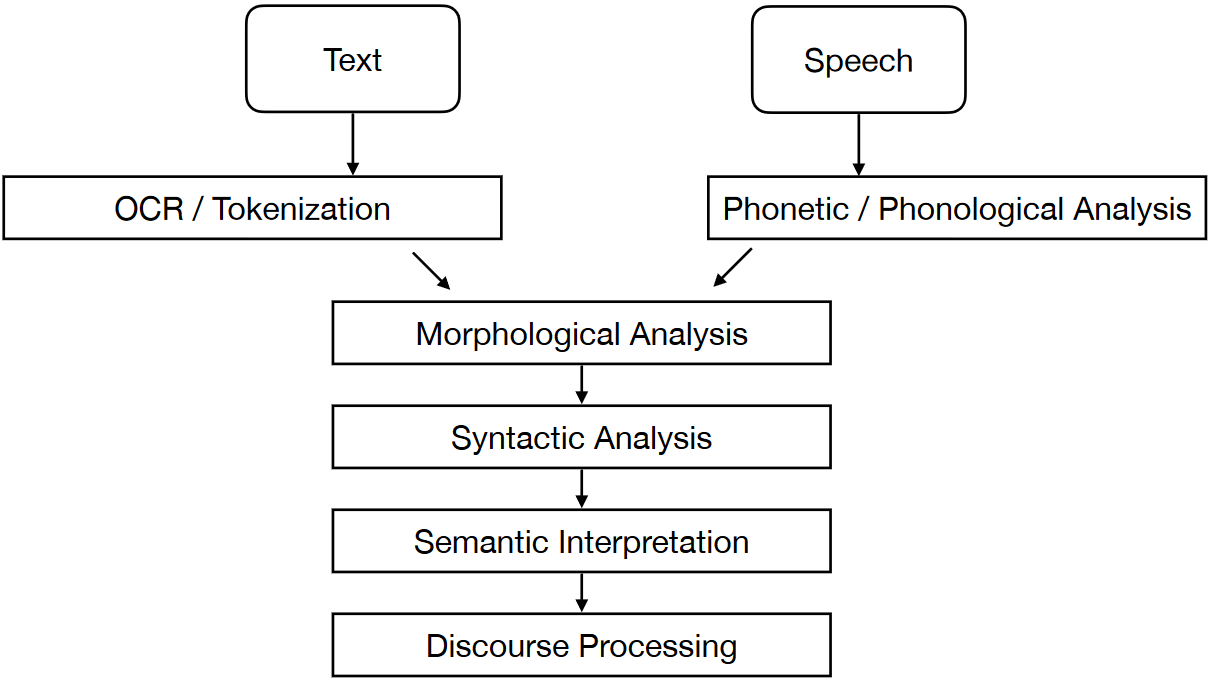
\includegraphics[width=0.9\textwidth]{images/NPL1.png} \\ \\
    \end{tabular}
\end{center}

\subsection{NLP Applications}
\begin{itemize}
    \item Spell checking, keyword search, finding synonyms
    \item Extracting information from documents or websites
    \item Text classification, reading level of school texts, sentiment analysis of longer documents
    \item Machine translation
    \item Conversational agents (spoken dialog)
    \item Question answering
\end{itemize}

\subsection{NLP Fundamental Tasks}
\begin{itemize}
    \item \textbf{Named entity recognition:} extrapolation and classification of particular words taken from a text within specific groups.
    \item \textbf{Entity mention detection:} classification of multiple entities into different groups.
    \item \textbf{Relation extraction:} association between different classes of vocabulary.
    \item \textbf{Coreference resolution:} association of a particular entity with a reference to it.
\end{itemize}

\subsection{Knowledge Acquisition}
NLP in terms of information seeking tasks:
\begin{itemize}
    \item Text classification
    \item Information retrieval
    \item Information extraction
\end{itemize}
A common factor in addressing these tasks is the use of language models, models that predict the probability distribution of language expressions.

\subsection{Language Models}
\begin{mdframed}
    \textbf{Language Models:} a (statistical) language model is a probability distribution over sequences of words.
\end{mdframed}
A formal language (Python) consists of strings specified by a set of rules called grammar.
The grammar defines which are the legal programs. \\
\vspace{1em}
Natural languages can not be characterized as a definitive set of sentences.
Natural languages are very large and ambiguous.

\subsection{The n-gram Model}
Given a written text, an n-gram model defines the probability of a sequence of characters:
\begin{equation} \tag*{}
    P(c_{1:N}) = \text{the probability of a sequence of } N \text{ characters, } c_1 \text{ up to } c_N
\end{equation}
A sequence of symbols of length n is an n-gram (there are special cases such as unigram, bigram, trigram, \ldots).
The unigram calculates the probability of only one character appearing, same goes for bigram and trigram only with 2 and 3 characters respectively.
Calculating this probability on large datasets gives the probability that various sequences will appear in natural language. \\
\vspace{1em}
An n-gram model is a Markov chain of order $n-1$.
In a Markov chain the probability of the character $c_i$ depends solely on the probability of the immediately preceding characters. \\
For example in a trigram (3-gram) model:
\begin{equation} \tag*{}
    P(c_i | c_{1:i-1}) = P(c_i | c_{i-2:i-1}) 
\end{equation}
We can define P(Ci:N) as a trigram using the chain rule and the Markov chain assumption:
\begin{equation} \tag*{}
    P(c_{1:N}) = \prod_{i=1}^N P(c_i | c_{1:i-1}) = \prod_{i=1}^N P(c_i | c_{i-2:i-1})
\end{equation}

\subsubsection{Language Identification}
This model is useful for language identification problems.
A simple approach can be based on creating a trigram model for each language:
\begin{equation} \tag*{}
    P(c_i | c_{i-2:i-1}, l)
\end{equation}
For each language the model is built by counting trigrams in a dataset of the specific language (about 100k characters needed).
Once this language is constructed, we can compute $P(\text{text}|\text{language})$.
Language identification then reduces to finding the $argmax$ of the function $P(l|c_{1:N})$. 
The probability of the language is estimated in other ways (extrapolating it from the data).

\subsubsection{Text Prediction}
Select the model that assigns a higher probability to the next word.
In this case the unigram model is not effective since context is important.

\subsubsection{Generative Models Using Word Models}
Using n-grams, one can define relationships between words, then select the highest probabilistic options to generate texts. \\
\vspace{1em}
A language model can be expressed in this way:
\begin{equation} \tag*{}
    P(w_n | w_1, w_2, \ldots, w_{i-1})
\end{equation}
and you can apply the chain rule to calculate the union of the probabilities of multiple words:
\begin{equation} \tag*{}
    P(w_1 w_2 \dots w_n) = \prod_i P(w_i | w_1 w_2 \ldots w_{i-1})
\end{equation}

\subsubsection{Text classification}
\ldots

\newpage